% lecture05.tex: Lecture 5: Atmospheres I, Composition, Structure, & Energy Balance
% Planetary Systems, Kapteyn Institute

\documentclass[aspectratio=169, 11pt]{beamer}

% ── Theme and macros ────────────────────────────────────────
\usepackage{../common/beamerthemeIPS}
% macros.tex: Shared math macros for IPS lecture slides
% Mirrors definitions in book/_config.yml for consistency
% Uses \providecommand to avoid conflicts with unicode-math

% ── Derivatives ─────────────────────────────────────────────
\providecommand{\dv}[2]{\frac{\mathrm{d} #1}{\mathrm{d} #2}}
\providecommand{\dd}{}\renewcommand{\dd}{\mathrm{d}}
\providecommand{\pdv}[2]{\frac{\partial #1}{\partial #2}}

% ── Solar quantities ────────────────────────────────────────
\newcommand{\Msun}{M_{\odot}}
\newcommand{\Rsun}{R_{\odot}}
\newcommand{\Lsun}{L_{\odot}}

% ── Planetary quantities ────────────────────────────────────
\newcommand{\Mearth}{M_{\oplus}}
\newcommand{\Rearth}{R_{\oplus}}
\newcommand{\Mjup}{M_{\mathrm{J}}}
\newcommand{\Rjup}{R_{\mathrm{J}}}

% ── Constants ───────────────────────────────────────────────
\newcommand{\kB}{k_{\mathrm{B}}}

% ── Media links ─────────────────────────────────────────────
% Clickable button that opens the animated or video version of a
% figure, e.g. \mediabutton{https://...gif}{Play animation}
\providecommand{\mediabutton}[2]{\href{#1}{\beamergotobutton{#2}}}

\graphicspath{{figures/}{../common/}{../../book/05_atmospheres_1/figures/}}

% ── Metadata ────────────────────────────────────────────────
\title[Lecture 5: Atmospheres I]{Lecture 5: Atmospheres I\\Composition, Structure, \& Energy Balance}
\subtitle{Planetary Systems}
\author[L5]{Mara Attia}
\institute{Kapteyn Astronomical Institute\\University of Groningen}
\date{2026}
\titlebgcredit{Earth's thin blue line, ISS STS-129 (2009). Credit: NASA}

% ════════════════════════════════════════════════════════════
\begin{document}

% ── Title slide ─────────────────────────────────────────────
\begin{frame}[plain,noframenumbering]
  \titlepage
\end{frame}

% ── Learning objectives ─────────────────────────────────────
\begin{frame}{Learning objectives}
  By the end of this lecture, you will be able to:
  \vskip8pt
  \begin{itemize}
    \item Classify atmospheric types (primary, secondary, tertiary)
    \item Derive pressure profiles from hydrostatic equilibrium
    \item Compute the atmospheric scale height and apply it across the solar system
    \item Explain how the greenhouse effect raises surface temperature above $T_{\mathrm{eff}}$
    \item Evaluate atmospheric escape mechanisms and retention criteria
  \end{itemize}
\end{frame}

% ── Recap ───────────────────────────────────────────────────
\begin{frame}{Recap: Lecture 4}
  \begin{itemize}
    \item Metal-silicate separation in magma oceans drove core formation within $\sim$30--60~Myr
    \item Dynamo requires conducting fluid, convection, and magnetic Reynolds number $\mathrm{Rm} \gtrsim 10$--100
    \item Mars lost its dynamo between $\sim$4.1 and 3.7~Ga, triggering atmospheric erosion
  \end{itemize}
  \vskip8pt
  \textbf{Today:} The thin gaseous envelope that controls a planet's surface conditions.
\end{frame}


% ════════════════════════════════════════════════════════════
\sectionimage{venera13_venus_surface}{The surface of Venus under its 92-bar atmosphere, Venera 13 (1982). Credit: USSR/NASA NSSDC, public domain}
\section{Atmospheric composition}
% ════════════════════════════════════════════════════════════

% ── Primary atmospheres ──────────────────────────────────────
\begin{frame}{Primary atmospheres}
  \textbf{Captured directly from the protoplanetary disk.}
  \vskip8pt
  \begin{itemize}
    \item Dominated by $\mathrm{H_2}$ and He (solar composition)
    \item Requires core mass $\gtrsim 5$--$10\;\Mearth$ before disk dispersal in $\sim$3--10~Myr
    \item \textbf{Gas giants:} Jupiter and Saturn retain massive $\mathrm{H_2}$/He envelopes
    \item \textbf{Ice giants:} Uranus and Neptune envelopes are only 10--20\% of total mass
    \item Terrestrial planets are too small to retain primordial $\mathrm{H_2}$/He
  \end{itemize}
\end{frame}

% ── Secondary atmospheres ────────────────────────────────────
\begin{frame}{Secondary atmospheres}
  \textbf{Produced by outgassing from the interior.}
  \vskip8pt
  \begin{itemize}
    \item Magma ocean degassing and volcanism release dissolved volatiles
    \item Speciation depends on mantle \textbf{oxygen fugacity} ($f_{\mathrm{O}_2}$ redox state):
    \begin{itemize}
      \item Oxidising: $\mathrm{CO_2}$, $\mathrm{H_2O}$, $\mathrm{N_2}$
      \item Reducing: $\mathrm{H_2}$, CO, $\mathrm{N_2}$
    \end{itemize}
    \item \textbf{Venus:} $\mathrm{CO_2}$-dominated (96.5\%), 92~bar
    \item \textbf{Mars:} $\mathrm{CO_2}$-dominated (95\%), 6~mbar
    \item \textbf{Titan:} thick $\mathrm{N_2}$ atmosphere (from $\mathrm{NH_3}$), 1.5~bar
  \end{itemize}
\end{frame}

% ── Tertiary atmospheres ─────────────────────────────────────
\begin{frame}{Tertiary atmospheres}
  Earth's atmosphere is a tertiary atmosphere produced by billions of years of biological modification.
  \vskip8pt
  \begin{itemize}
    \item Original outgassed inventory was dominated by $\mathrm{CO_2}$ and $\mathrm{N_2}$, similar to Venus
    \item Oxygenic photosynthesis added the $\mathrm{O_2}$ (21\%); the $\mathrm{N_2}$ (78\%) is outgassed and accumulated
    \item Atmospheric $\mathrm{O_2}$ is entirely biogenic and requires active life to persist
  \end{itemize}
  \vskip8pt
    \keyresult{Earth's $\mathrm{O_2}$, and so its tertiary character, is continuously maintained by life.}
\end{frame}

% ── Comparative table ────────────────────────────────────────
\begin{frame}{Comparative atmospheric properties}
  \centering
  \small
  \begin{tabular}{l c c c c c}
    \toprule
    & \textbf{Venus} & \textbf{Earth} & \textbf{Mars} & \textbf{Jupiter} & \textbf{Titan} \\
    \midrule
    $P_{\mathrm{surf}}$ (bar) & 92 & 1.0 & 0.006 & n/a & 1.5 \\
    $T_{\mathrm{surf}}$ (K)   & 737 & 288 & 215 & n/a & 94 \\
    Dominant gas              & $\mathrm{CO_2}$ & $\mathrm{N_2}$ & $\mathrm{CO_2}$ & $\mathrm{H_2}$ & $\mathrm{N_2}$ \\
    Secondary gas             & $\mathrm{N_2}$ & $\mathrm{O_2}$ & $\mathrm{N_2}$ & He & $\mathrm{CH_4}$ \\
    $\mu$                     & 43.4 & 28.97 & 43.3 & 2.2 & 28.6 \\
    Type                      & 2$^{\circ}$ & 3$^{\circ}$ & 2$^{\circ}$ & 1$^{\circ}$ & 2$^{\circ}$ \\
    \bottomrule
  \end{tabular}
  \vskip8pt
  Staggering diversity: surface pressures spanning five orders of magnitude, temperatures from 94 to 737~K.
\end{frame}

% ── Composition bars hero ────────────────────────────────────
\begin{frame}
  \centering
  \makebox[\linewidth][c]{\includegraphics[width=0.95\paperwidth, height=0.72\paperheight, keepaspectratio]{composition_bar}}\\
  {\footnotesize Atmospheric composition by volume for five solar-system bodies: three origins yield five distinct outcomes across the solar system. Course figure.}
\end{frame}

% ── Venus surface ────────────────────────────────────────────
\begin{frame}{Venus: a secondary atmosphere in extremis}
  A massive secondary atmosphere transforms planetary surface conditions to extreme pressures and temperatures.
  \vskip6pt
  \begin{columns}[c]
    \column{\recapfigcolnarrow}
    \centering
    \ipsrecapfig{venera13_venus_surface}
    \source{USSR/NASA NSSDC, public domain}

    \column{\recaptextcolwide}
    \begin{itemize}
      \item \textit{Venera 13} landed 1 March 1982 and survived 127~minutes
      \item Surface pressure of 92~bar and surface temperature of 737~K
      \item Dense $\mathrm{CO_2}$ atmosphere and cloud deck filter sunlight to a dim orange glow
    \end{itemize}
  \end{columns}
\end{frame}


% ════════════════════════════════════════════════════════════
\sectionimage{mars_atmosphere}{The thin atmosphere of Mars above its limb, Viking 1 (1976). Credit: NASA/JPL}
\section{Hydrostatic equilibrium}
% ════════════════════════════════════════════════════════════

% ── Hydrostatic equilibrium ──────────────────────────────────
\begin{frame}{Hydrostatic equilibrium}
  \begin{columns}[c]
    \column{\recapfigcol}
    \ipsrecapfig{hydrostatic_slab}
    \source{Course figure}

    \column{\recaptextcol}
    \small
    Net vertical force on a thin slab of area $A$ and thickness $\dd z$ vanishes:
    $$P(z)A - P(z + \dd z)A = \rho\,g\,A\,\dd z$$
    \vskip4pt
    \keyresult{$$\boxed{\dv{P}{z} = -\rho\,g}$$}
    \vskip4pt
    Pressure decreases upward because each layer supports the weight of all gas above it.
  \end{columns}
\end{frame}

% ── Ideal gas law & barometric formula ───────────────────────
\begin{frame}{The ideal gas law and barometric formula}
  The ideal gas law relates density to pressure: $P = \rho\,\kB T / (\mu\,m_u)$.
  \vskip6pt
  Substituting $\rho(P)$ into hydrostatic equilibrium $\dv{P}{z} = -\rho\,g$:
  $$\dv{P}{z} = -\frac{\mu\,m_u\,g}{\kB T}\,P = -\frac{P}{H}$$
  \vskip4pt
  For an \textbf{isothermal} atmosphere (constant $T$), integrating yields:
  \vskip4pt
  \keyresult{$$\boxed{P(z) = P_0\,\exp\!\left(-\frac{z}{H}\right)}$$}
  \vskip4pt
  where $H = \kB T/(\mu\,m_u\,g)$; pressure drops by $e \approx 2.718$ each scale height.
\end{frame}


% ════════════════════════════════════════════════════════════
\sectionimage{title_background}{Sunrise over Earth's limb from orbit. Credit: NASA}
\section{Blackboard derivation: scale height}
% ════════════════════════════════════════════════════════════

% ── Setup ────────────────────────────────────────────────────
\begin{frame}{Deriving the scale height}
  \textbf{Goal:} Derive $H = \kB T/(\mu\,m_u\,g)$ from hydrostatic equilibrium and the ideal gas law.
  \vskip10pt
  Start from:
  $$\dv{P}{z} = -\rho\,g \qquad\text{and}\qquad P = \frac{\rho\,\kB T}{\mu\,m_u}$$
  \vskip6pt
  Express $\rho$ in terms of $P$:
  $$\rho = \frac{P\,\mu\,m_u}{\kB T}$$
  \vskip4pt
  Substitute:
  $$\dv{P}{z} = -\frac{\mu\,m_u\,g}{\kB T}\,P \equiv -\frac{P}{H}$$
\end{frame}

% ── Result ───────────────────────────────────────────────────
\begin{frame}{The atmospheric scale height}
  \keyresult{$$\boxed{H = \frac{\kB T}{\mu\,m_u\,g}}$$}
  \vskip8pt
  Physical interpretation:
  \vskip4pt
  \begin{itemize}
    \item \textbf{Higher $T$} $\rightarrow$ larger $H$: hotter gas extends further
    \item \textbf{Heavier molecules} (larger $\mu$) $\rightarrow$ smaller $H$: harder to loft
    \item \textbf{Stronger gravity} $g$ $\rightarrow$ smaller $H$: more compressed
  \end{itemize}
  \vskip8pt
  \textbf{Key insight:} $H$ encodes the competition between thermal energy and gravitational binding; integrated over the whole column, the surface pressure is the column weight, $P_0 = m_{\mathrm{col}}\,g$.
\end{frame}

% ── Scale heights across the solar system ────────────────────
\begin{frame}{Scale heights across the solar system}
  \centering
  \begin{tabular}{l c c c c}
    \toprule
    \textbf{Body} & $\boldsymbol{T}$~\textbf{(K)} & $\boldsymbol{\mu}$ & $\boldsymbol{g}$~\textbf{(m\,s$^{-2}$)} & $\boldsymbol{H}$~\textbf{(km)} \\
    \midrule
    Venus   & 737  & 43.4 & 8.87  & 15.9 \\
    Earth   & 288  & 28.97 & 9.81  & 8.4  \\
    Mars    & 215  & 43.3 & 3.72  & 11.1 \\
    Jupiter & 165  & 2.2  & 24.8  & 25   \\
    Titan   & 94   & 28.6 & 1.35  & 20   \\
    \bottomrule
  \end{tabular}
  \vskip10pt
  \begin{itemize}
    \item Jupiter: large $H$ despite strong gravity, because $\mathrm{H_2}$ is very light ($\mu = 2.2$)
    \item Titan: large $H$ despite low $T$, thanks to very weak gravity ($g = 1.35$~m\,s$^{-2}$)
    \item Venus: hot but heavy molecules and decent gravity yield moderate $H$
  \end{itemize}
\end{frame}


% ════════════════════════════════════════════════════════════
\sectionimage{earth_tz_layers}{Earth's atmospheric layers. Course figure}
\section{Vertical structure}
% ════════════════════════════════════════════════════════════

% ── Atmospheric layers ───────────────────────────────────────
\begin{frame}{Atmospheric layers}
  \begin{columns}[c]
    \column{\recapfigcolnarrow}
    \centering
    \ipsrecapfig[0.65\textheight]{earth_tz_layers}
    \source{Course figure; US Standard Atmosphere 1976}

    \column{\recaptextcolwide}
    \small
    Layers defined by the sign of $\dv{T}{z}$:
    \vskip2pt
    \begin{enumerate}
      \item \textbf{Troposphere} (0--12~km): $T$ decreases with $z$; convective
      \item \textbf{Stratosphere} (12--50~km): $T$ increases; UV ozone heating
      \item \textbf{Mesosphere} (50--85~km): $T$ decreases to mesopause ($\sim$190~K)
      \item \textbf{Thermosphere} ($>$85~km): $T$ increases; EUV heating ($T > 1000$~K)
    \end{enumerate}
  \end{columns}
\end{frame}

% ── Lapse rate ───────────────────────────────────────────────
\begin{frame}{The adiabatic lapse rate}
  In the troposphere, convection sets the temperature gradient:
  \vskip6pt
  \keyresult{$$\Gamma_d = -\dv{T}{z} = \frac{g}{c_p}$$}
  \vskip6pt
  \begin{itemize}
    \item \textbf{Dry adiabatic lapse rate} for Earth: $\Gamma_d = 9.81/1004 \approx 9.8$~K\,km$^{-1}$
    \item Observed average: $\sim$6.5~K\,km$^{-1}$ (lower due to latent heat release)
    \item Physical picture: rising air expands, does work on surroundings, cools
  \end{itemize}
  \vskip6pt
  \textbf{Tropopause height:} $\sim$8~km (poles) to $\sim$17~km (equator).
\end{frame}

% ── Dry and moist adiabat hero ───────────────────────────────
\begin{frame}
  \centering
  \makebox[\linewidth][c]{\includegraphics[width=0.95\paperwidth, height=0.72\paperheight, keepaspectratio]{dry_moist_adiabat}}\\
  {\footnotesize Dry and moist adiabats against the US Standard Atmosphere 1976 reference profile: latent heat makes the moist adiabat shallower, and real convection sits between both limits. Course figure.}
\end{frame}

% ── Titan descent profile hero ───────────────────────────────
\begin{frame}
  \centering
  \makebox[\linewidth][c]{\includegraphics[width=0.95\paperwidth, height=0.72\paperheight, keepaspectratio]{fulchignoni2005_titan_tz}}\\
  {\footnotesize Titan's temperature profile from the Huygens HASI descent: an in situ descent measured the 94~K surface, 0.1~bar tropopause, and stratospheric structure. Fulchignoni et al.\ (2005).}
\end{frame}

% ── Venus profile hero ───────────────────────────────────────
\begin{frame}
  \centering
  \makebox[\linewidth][c]{\includegraphics[width=0.95\paperwidth, height=0.72\paperheight, keepaspectratio]{venus_tz_vira}}\\
  {\footnotesize Venus temperature profile, Pioneer Venus/VIRA and Venus Express: without ozone, temperature falls monotonically from 737~K at the surface to the mesopause, reaching 1~bar near 50~km. Course figure.}
\end{frame}

% ── Seven atmospheres 0.1-bar hero ───────────────────────────
\begin{frame}
  \centering
  \makebox[\linewidth][c]{\includegraphics[width=0.95\paperwidth, height=0.72\paperheight, keepaspectratio]{atmosphere_tp_robinson}}\\
  {\footnotesize Measured temperature-pressure profiles of seven solar-system atmospheres: thick atmospheres transition from convective to radiative near 0.1~bar, setting a universal tropopause minimum. Digitized from Robinson \& Catling (2014), Fig.\ 1.}
\end{frame}


% ════════════════════════════════════════════════════════════
\sectionimage{blackbody_spectrum}{Blackbody spectra. Credit: Wikimedia, public domain}
\section{Radiative transfer basics}
% ════════════════════════════════════════════════════════════

% ── Absorption, emission, scattering ─────────────────────────
\begin{frame}{Three interactions: radiation and matter}
  When radiation passes through an atmosphere:
  \vskip8pt
  \begin{description}
    \item[Absorption:] Photon energy converted to internal molecular energy\\
    Key absorbers: $\mathrm{CO_2}$, $\mathrm{H_2O}$, $\mathrm{CH_4}$, $\mathrm{O_3}$, $\mathrm{N_2O}$

    \vskip4pt
    \item[Emission:] Warm gas radiates at absorbed wavelengths (Kirchhoff's law)\\
    Radiates energy directly to space

    \vskip4pt
    \item[Scattering:] Photons redirected without absorption\\
    Rayleigh scattering ($\propto \lambda^{-4}$) and Mie scattering
  \end{description}
\end{frame}

% ── Blackbody spectrum figure ────────────────────────────────
\begin{frame}{Stellar vs.\ planetary emission}
  \begin{columns}[c]
    \column{\recapfigcol}
    \centering
    \ipsrecapfig{blackbody_spectrum}
    \source{Wikimedia, public domain}

    \column{\recaptextcol}
    \begin{itemize}
      \item Sun ($\sim$5800~K): peak at $\sim$0.5~$\mu$m (visible)
      \item Planet ($\sim$300~K): peak at $\sim$10~$\mu$m (thermal IR)
    \end{itemize}
    \vskip6pt
    This \textbf{wavelength separation} is the physical basis of the greenhouse effect: the atmosphere can be transparent at visible wavelengths but opaque in the infrared.
  \end{columns}
\end{frame}

% ── Optical depth & Beer-Lambert law ─────────────────────────
\begin{frame}{Optical depth and the Beer-Lambert law}
  Optical depth $\tau$ measures cumulative absorption along a path:
  $$\tau = \int_0^s \kappa\,\rho\,\dd s'$$
  \vskip2pt
  Beam intensity decays following the \textbf{Beer-Lambert law}:
  \vskip2pt
  \keyresult{$$\boxed{I = I_0\,e^{-\tau}}$$}
  \vskip4pt
  \begin{itemize}
    \item \textbf{Optically thin} ($\tau \ll 1$): radiation passes freely through the gas
    \item \textbf{Optically thick} ($\tau \gg 1$): photons are repeatedly absorbed and re-emitted
    \item \textbf{Photosphere} ($\tau \approx 1$): thermal radiation escapes directly to space
  \end{itemize}
\end{frame}

% ── Photosphere schematic hero ───────────────────────────────
\begin{frame}
  \centering
  \makebox[\linewidth][c]{\includegraphics[width=0.95\paperwidth, height=0.72\paperheight, keepaspectratio]{tau_one_schematic}}\\
  {\footnotesize The atmospheric photosphere: thermal radiation escapes to space from the $\tau \approx 1$ level, setting the effective temperature. Course figure.}
\end{frame}

% ── Atmospheric absorption spectrum hero ─────────────────────
\begin{frame}
  \centering
  \makebox[\linewidth][c]{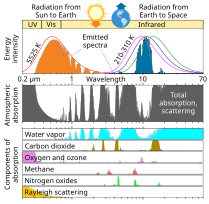
\includegraphics[width=0.95\paperwidth, height=0.72\paperheight, keepaspectratio]{atmospheric_transmission}}\\
  {\footnotesize Earth's atmospheric absorption spectrum from UV to IR: greenhouse gases absorb outgoing surface infrared while leaving visible sunlight and the 8--13~$\mu$m window transparent. Credit: Wikimedia Commons, public domain.}
\end{frame}


% ── Break ───────────────────────────────────────────────────
\breakslide


% ════════════════════════════════════════════════════════════
\sectionimage{greenhouse_one_layer}{The one-layer greenhouse model. Course figure}
\section{Energy balance \& greenhouse effect}
% ════════════════════════════════════════════════════════════

% ── Radiative-convective equilibrium ─────────────────────────
\begin{frame}{Radiative-convective equilibrium}
  Atmospheres divide into a convective lower layer and a radiatively controlled upper layer.
  \vskip6pt
  \begin{itemize}
    \item \textbf{Troposphere}: greenhouse opacity drives convective instability along the adiabat
    \item \textbf{Stratosphere}: optically thin gas reaches radiative equilibrium, stable against convection
    \item \textbf{Tropopause}: boundary where the radiative temperature gradient becomes shallower than the adiabat
  \end{itemize}
\end{frame}

% ── Energy balance derivation ────────────────────────────────
\begin{frame}{Planetary energy balance}
  Absorbed stellar power equals emitted thermal radiation:
  $$(1-A)\frac{S}{4} = \sigma\,T_{\mathrm{eff}}^4 \qquad\text{where}\quad S = \frac{L_\star}{4\pi d^2}$$
  \vskip4pt
  \begin{itemize}
    \item $A$: Bond albedo; $S$: stellar flux ($S_0 = 1361$~W\,m$^{-2}$ at Earth)
    \item Factor $1/4$: ratio of intercepting cross-section $\pi R_p^2$ to emitting sphere $4\pi R_p^2$
  \end{itemize}
  \vskip6pt
  \keyresult{$$\boxed{T_{\mathrm{eff}} = \left[\frac{(1-A)\,L_\star}{16\pi\sigma\,d^2}\right]^{1/4} = \left[\frac{(1-A)\,S}{4\sigma}\right]^{1/4}}$$}
\end{frame}

% ── Earth energy budget hero ─────────────────────────────────
\begin{frame}
  \centering
  \makebox[\linewidth][c]{\includegraphics[width=0.95\paperwidth, height=0.72\paperheight, keepaspectratio]{trenberth_energy_budget}}\\
  {\footnotesize Earth's globally averaged energy budget in W\,m$^{-2}$: atmospheric back-radiation of 333~W\,m$^{-2}$ supplies more energy to the surface than direct sunlight (160~W\,m$^{-2}$). After Trenberth et al.\ (2009).}
\end{frame}

% ── Effective vs surface T ───────────────────────────────────
\begin{frame}{Effective vs.\ surface temperature}
  \centering
  \begin{tabular}{l c c c c c}
    \toprule
    \textbf{Body} & $\boldsymbol{A}$ & $\boldsymbol{d}$~\textbf{(AU)} & $\boldsymbol{T_{\mathrm{eff}}}$~\textbf{(K)} & $\boldsymbol{T_{\mathrm{surf}}}$~\textbf{(K)} & $\boldsymbol{\Delta T}$~\textbf{(K)} \\
    \midrule
    Venus   & 0.77 & 0.72 & 227 & 737  & +510 \\
    Earth   & 0.30 & 1.00 & 255 & 288  & +33  \\
    Mars    & 0.25 & 1.52 & 210 & 215  & +5 \\
    Jupiter & 0.34 & 5.20 & 110 & 165* & +55  \\
    \bottomrule
  \end{tabular}
  \vskip4pt
  {\footnotesize *Jupiter 1-bar level; excess partly from internal heat (Lecture~3).}
  \vskip8pt
  $\Delta T = T_{\mathrm{surf}} - T_{\mathrm{eff}}$ reveals the \textbf{greenhouse effect}.\\
  Venus: 510~K. Earth: 33~K. Mars: $\sim$5~K (only 6~mbar, no water-vapour amplifier).
\end{frame}

% ── Greenhouse mechanism ─────────────────────────────────────
\begin{frame}{The greenhouse mechanism}
  \begin{columns}[c]
    \column{\recapfigcolnarrow}
    \centering
    \ipsrecapfig{greenhouse_one_layer}
    \source{Course figure}

    \column{\recaptextcolwide}
    \begin{enumerate}
      \item Sunlight (visible, $\sim$0.5~$\mu$m) reaches the surface
      \item Surface emits thermal IR ($\sim$10--15~$\mu$m)
      \item Greenhouse gases absorb outgoing IR
      \item Absorbing layer re-emits: half up, half down
      \item Downward emission adds energy to surface
    \end{enumerate}
    \vskip6pt
    \textbf{Result:} $T_{\mathrm{surf}} > T_{\mathrm{eff}}$
  \end{columns}
\end{frame}

% ── One-layer greenhouse model ───────────────────────────────
\begin{frame}{One-layer greenhouse model}
  Single atmospheric layer with infrared emissivity $\varepsilon$, transparent to visible sunlight:
  \vskip4pt
  \begin{columns}[T]
    \column{0.48\textwidth}
    \textbf{Flux balance:}
    \begin{align*}
      \text{Atmosphere:} & \quad \varepsilon\sigma T_s^4 = 2\varepsilon\sigma T_a^4 \\
      \text{Surface:} & \quad (1-A)\frac{F_\star}{4} + \varepsilon\sigma T_a^4 = \sigma T_s^4 \\
      \text{TOA:} & \quad (1-A)\frac{F_\star}{4} = \sigma T_{\mathrm{eff}}^4
    \end{align*}

    \column{0.48\textwidth}
    \textbf{Surface temperature:}
    \keyresult{$$\boxed{T_s = T_{\mathrm{eff}}\left(\frac{2}{2-\varepsilon}\right)^{1/4}}$$}
  \end{columns}
  \vskip6pt
  \begin{itemize}
    \item $\varepsilon = 0$ (transparent): $T_s = T_{\mathrm{eff}}$
    \item $\varepsilon = 1$ (opaque): $T_s = 2^{1/4}\,T_{\mathrm{eff}} \approx 1.19\,T_{\mathrm{eff}}$ (Earth: $\approx$303~K)
  \end{itemize}
\end{frame}


% ════════════════════════════════════════════════════════════
\sectionimage{escape_processes_gronoff2020}{The main atmospheric escape processes. Gronoff et al.\ (2020)}
\section{Atmospheric escape}
% ════════════════════════════════════════════════════════════

% ── Jeans escape ─────────────────────────────────────────────
\begin{frame}{Thermal (Jeans) escape}
  Molecules follow a Maxwell-Boltzmann distribution whose high-velocity tail can exceed escape speed.
  \vskip6pt
  The \textbf{Jeans escape parameter} at the exobase compares gravitational to thermal energy:
  \vskip4pt
  \keyresult{$$\lambda_J = \frac{G M_p\,m}{\kB T_{\mathrm{exo}}\,r_{\mathrm{exo}}} = \frac{v_{\mathrm{esc}}^2}{v_{\mathrm{th}}^2}$$}
  \vskip2pt
  with $v_{\mathrm{th}} = \sqrt{2\kB T_{\mathrm{exo}}/m}$ the most probable thermal speed.
  \vskip6pt
  \begin{itemize}
    \item $\lambda_J \gg 1$: escape is negligible because the tail is depleted
    \item $\lambda_J \lesssim 2$--3: thermal escape drives rapid atmospheric loss
    \item Escape flux $\Phi_J \propto (1 + \lambda_J)\,e^{-\lambda_J}$ depends exponentially on $\lambda_J$
  \end{itemize}
\end{frame}

% ── Escape processes hero ────────────────────────────────────
\begin{frame}
  \centering
  \makebox[\linewidth][c]{\includegraphics[width=0.95\paperwidth, height=0.72\paperheight, keepaspectratio]{escape_processes_gronoff2020}}\\
  {\footnotesize The main atmospheric escape processes: thermal, photochemical, and ion channels operate on all planets, while planetary magnetic fields select which pathways dominate. Gronoff et al.\ (2020).}
\end{frame}

% ── Jeans parameter table ────────────────────────────────────
\begin{frame}{Jeans parameter for Earth and Mars}
  Because $\lambda_J \propto m$, light hydrogen escapes steadily while heavy molecules remain gravitationally bound.
  \vskip4pt
  \centering
  {\footnotesize Exobase temperatures: 1000~K (Earth), 270~K (Mars).}
  \vskip4pt
  \small
  \begin{tabular}{l c c c}
    \toprule
    \textbf{Species} & $\boldsymbol{m}$~\textbf{(u)} & $\boldsymbol{\lambda_J}$~\textbf{(Earth)} & $\boldsymbol{\lambda_J}$~\textbf{(Mars)} \\
    \midrule
    H               & 1  & 7.0  & 5.3  \\
    $\mathrm{H_2}$  & 2  & 14   & 11   \\
    He              & 4  & 28   & 21   \\
    $\mathrm{N_2}$  & 28 & 200  & 150  \\
    $\mathrm{CO_2}$ & 44 & 310  & 230  \\
    \bottomrule
  \end{tabular}
  \vskip4pt
  \flushleft
  \begin{itemize}
    \item $\lambda_J \gg 1$ for $\mathrm{N_2}$ and $\mathrm{CO_2}$: thermal escape is completely negligible
    \item Moderate $\lambda_J$ allows atomic H to escape steadily from both planets
  \end{itemize}
\end{frame}

% ── Exobase crossing hero ────────────────────────────────────
\begin{frame}
  \centering
  \makebox[\linewidth][c]{\includegraphics[width=0.95\paperwidth, height=0.72\paperheight, keepaspectratio]{exobase_definition}}\\
  {\footnotesize The exobase: altitude where the mean free path $\ell$ equals the scale height $H$, splitting collisional fluid below from ballistic flight above. Course figure.}
\end{frame}

% ── Exobase speed distributions hero ─────────────────────────
\begin{frame}
  \centering
  \makebox[\linewidth][c]{\includegraphics[width=0.95\paperwidth, height=0.72\paperheight, keepaspectratio]{maxwell_boltzmann_jeans}}\\
  {\footnotesize Maxwell-Boltzmann speed distributions for atomic H at Earth and Mars exobases: the escaping fraction sits in the high-velocity tail exceeding $v_{\mathrm{esc}}$, scaling as $e^{-\lambda_J}$. Course figure.}
\end{frame}

% ── Hydrodynamic escape ─────────────────────────────────────
\begin{frame}{Hydrodynamic escape}
  Intense stellar EUV heating drives bulk outflow as an \textbf{atmospheric wind}:
  \vskip8pt
  \begin{itemize}
    \item Peak importance in first few hundred Myr when stellar EUV is 10--100$\times$ higher
    \item Strips $\mathrm{H_2}$-rich primary envelopes from planets up to several $\Mearth$
    \item Outflowing light hydrogen can drag along heavier volatiles (He, C, N, O)
    \item Primary mechanism sculpting the exoplanet radius valley at $\sim$1.5--2~$\Rearth$
  \end{itemize}
  \vskip4pt
  \sourcenote{Hunten et al.\ (1987); Owen (2019)}
\end{frame}

% ── Radius valley hero ───────────────────────────────────────
\begin{frame}
  \centering
  \makebox[\linewidth][c]{\includegraphics[width=0.95\paperwidth, height=0.72\paperheight, keepaspectratio]{fulton2017_radius_valley}}\\
  {\footnotesize The observed radius valley in the California-Kepler Survey: a bimodal distribution with a deficit near 1.8~$\Rearth$ separates stripped rocky cores from envelope-retaining sub-Neptunes. After Fulton et al.\ (2017).}
\end{frame}

% ── Energy-limited escape ────────────────────────────────────
\begin{frame}{Energy-limited escape rate}
  Stellar EUV energy absorbed in the upper atmosphere drives hydrodynamic mass loss in the energy-limited regime.
  \vskip6pt
  \keyresult{$$\dot{M}_{\mathrm{EL}} = \eta\,\frac{\pi\,F_\mathrm{EUV}\,R_p^3}{G\,M_p}$$}
  \vskip6pt
  \begin{itemize}
    \item Efficiency $\eta \approx 0.1$--$0.2$ converts incident EUV flux into expansion work
    \item Scales as $R_p^3$: extended, low-density atmospheres lose mass most rapidly
    \item Scales inversely with $M_p$: lower planetary gravity enables stronger bulk outflow
  \end{itemize}
  \vskip4pt
  \sourcenote{Watson et al.\ (1981); Owen (2019)}
\end{frame}

% ── Non-thermal escape ───────────────────────────────────────
\begin{frame}{Non-thermal escape mechanisms}
  \begin{description}
    \item[Sputtering:] Solar wind ions strike upper atmosphere and eject neutral molecules
    \vskip2pt
    \item[Photochemical:] Photodissociation yields suprathermal atoms exceeding $v_{\mathrm{esc}}$
    \vskip2pt
    \item[Ion pickup:] Photoions are swept away by interplanetary magnetic fields
    \vskip2pt
    \item[Impact erosion:] Giant impacts shock and eject atmospheric columns into space
  \end{description}
  \vskip6pt
  {\small MAVEN at Mars: photochemical loss of oxygen dominates modern escape over sputtering and ion pickup.}
\end{frame}

% ── Oxygen loss channels hero ────────────────────────────────
\begin{frame}
  \centering
  \makebox[\linewidth][c]{\includegraphics[width=0.95\paperwidth, height=0.72\paperheight, keepaspectratio]{maven_o_loss_channels}}\\
  {\footnotesize Present-day oxygen loss from Mars by escape channel: photochemical escape dominates modern oxygen loss; summed with hydrogen escape, the total reaches the 2--3~kg\,s$^{-1}$ MAVEN measures. After Jakosky et al.\ (2018).}
\end{frame}


% ════════════════════════════════════════════════════════════
\sectionimage{escape_velocity_temperature}{Escape velocity vs.\ temperature. Credit: Wikimedia, CC BY-SA 4.0}
\section{Atmospheric retention}
% ════════════════════════════════════════════════════════════

% ── Escape velocity–temperature diagram ──────────────────────
\begin{frame}{Atmospheric retention: $v_{\mathrm{esc}}$ vs.\ $T$ diagram}
  \begin{columns}[c]
    \column{\recapfigcolnarrow}
    \centering
    \ipsrecapfig{escape_velocity_temperature}
    \source{Wikimedia, CC BY-SA 4.0}

    \column{\recaptextcolwide}
    Rule of thumb for long-term retention:
    $$v_{\mathrm{esc}} \gtrsim 6\,v_{\mathrm{th}}$$
    \vskip4pt
    \begin{itemize}
      \item Gas giants: retain all species
      \item Earth/Venus: retain heavy species, lose H
      \item Mars: marginal; non-thermal losses dominate
      \item Titan: cold $\rightarrow$ retains $\mathrm{N_2}$ despite low $v_{\mathrm{esc}}$
      \item Moon/Mercury: retain no significant atmosphere
    \end{itemize}
  \end{columns}
\end{frame}

% ── Mars atmosphere ──────────────────────────────────────────
\begin{frame}{Mars: a lost atmosphere}
  Loss of Mars' magnetic dynamo allowed solar wind stripping to erode an early thick atmosphere down to 6~mbar.
  \vskip6pt
  \begin{columns}[c]
    \column{\recapfigcolnarrow}
    \centering
    \ipsrecapfig[0.6\textheight]{mars_atmosphere}
    \source{NASA/JPL (Viking 1, 1976)}

    \column{\recaptextcolwide}
    \begin{itemize}
      \item Today 6~mbar: no stable liquid water, little greenhouse warming
      \item Valley networks and lakes record a dense early atmosphere
      \item The dynamo died near $\sim$4.1~Ga and left the atmosphere to the solar wind
    \end{itemize}
  \end{columns}
\end{frame}


% ════════════════════════════════════════════════════════════
\sectionimage{earth_thin_blue_line}{Earth's atmosphere. Credit: NASA/ISS}
\section{Recent advances \& outlook}
% ════════════════════════════════════════════════════════════

% ── TRAPPIST-1 b emission hero ───────────────────────────────
\begin{frame}
  \centering
  \makebox[\linewidth][c]{\includegraphics[width=0.95\paperwidth, height=0.72\paperheight, keepaspectratio]{trappist1b_jwst_greene2023}}\\
  {\footnotesize JWST/MIRI 15~$\mu$m thermal emission matches a 503~K bare rock, ruling out a thick atmosphere on TRAPPIST-1~b. Greene et al.\ (2023).}
\end{frame}

% ── Summary ──────────────────────────────────────────────────
\begin{frame}{Summary}
  \small
  \begin{enumerate}\setlength\itemsep{1pt}
    \item \textbf{Atmosphere types}: primary (captured), secondary (outgassed), tertiary (biogenic)
    \item \textbf{Hydrostatic balance}: $\dv{P}{z} = -\rho g$ yields exponential pressure decay $P_0 e^{-z/H}$
    \item \textbf{Scale height}: $H = \kB T/(\mu m_u g)$ balances thermal energy against gravity
    \item \textbf{Vertical structure}: convection sets the lapse rate ($\Gamma_d = g/c_p$ dry, less when condensing) below the 0.1~bar tropopause
    \item \textbf{Beer-Lambert law}: $I = I_0 e^{-\tau}$; thermal radiation escapes from photosphere at $\tau \approx 1$
    \item \textbf{Greenhouse warming}: optical depth raises surface temperature $T_s$ above $T_{\mathrm{eff}}$
    \item \textbf{Atmospheric escape}: thermal, hydrodynamic, and non-thermal; retention requires $v_{\mathrm{esc}} \gtrsim 6 v_{\mathrm{th}}$
  \end{enumerate}
  \vskip4pt
  \textbf{Next: Lecture 6}
\end{frame}

% ── Final slide ─────────────────────────────────────────────
\begin{frame}[plain,noframenumbering]
  \begin{tikzpicture}[remember picture, overlay]
    \ipscontain{title_background}
    \fill[ipsPrimary, opacity=0.70] (current page.north west) rectangle (current page.south east);
  \end{tikzpicture}
  \vfill
  \begin{center}
    {\color{white}\Large\bfseries Questions?}
    \vskip20pt
    {\color{white!85}\large Next: Lecture 6, Atmospheres II: clouds, weather \& climate (Mara Attia)}\\[4pt]
    {\color{white!85}\small Thu 24 Sep, 11:00--13:00, room 5419.0161 (Collegezaal)}\\[12pt]
    {\color{white!85}\small Next tutorial: Fri 25 Sep, 13:00--15:00, room 5419.0161 (Collegezaal)}\\[20pt]
    {\color{white!70}\small \texttt{https://ips.formingworlds.space}}
  \end{center}
  \vfill
\end{frame}

\end{document}
